\documentclass[a4paper,10pt]{scrartcl}

\usepackage{polski}
\usepackage[utf8]{inputenc}
\usepackage{graphicx}

\title{}
\author{}
\date{}

\pdfinfo{%
  /Title    (lab1)
  /Author   (Filip Malinowski)
}

\begin{document}

\title{Sprawozdanie z lab1}
\author{Filip Malinowski}
\date{\today}

\maketitle

W zadaniu są dwa programy. Pierwszy generuje dane wejściowe.
Drugi, właściwy uruchamia algorytm mnożenia każdego elementu
tablicy przez 2. Oba programy uruchamiane są przez Makefile.
W tej wersji nie wspiera różnej ilości danych wejściowych.
Program testujący algorytm składa się z klasy bazowej
Benchmark i klasy pochodnej Mnożenie. Klasa Benchmark ma
zdefiniowaną metodę testowania szybkości działania
algorytmów. W tej metodzie czas jest wyznaczany za pomocą
high resolution clock z biblioteki chrono. Następie tworzony
jest plik wyjściowy, do którego zapisywane są dane o ilości
testowanych elementów oraz czasie wykonywania algorytmu.

Załączony wykres szybkości działania algorytmu:

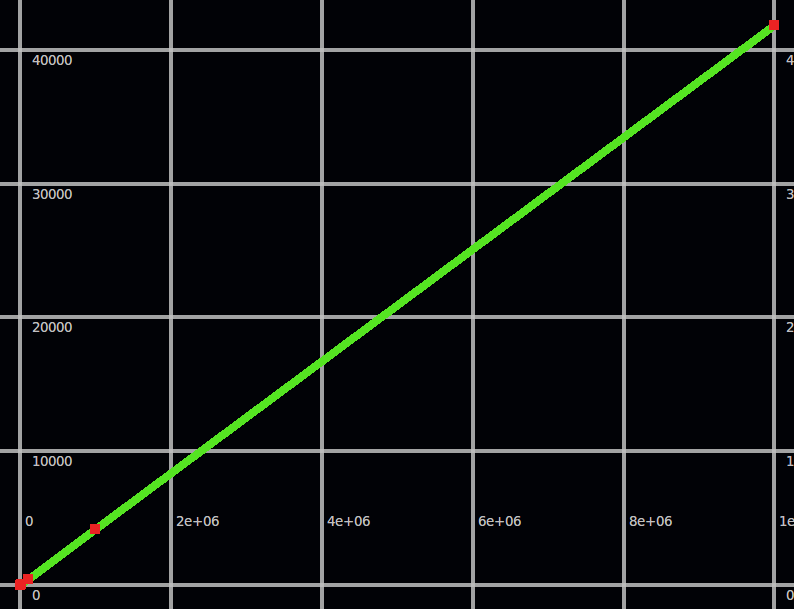
\includegraphics[scale=0.3]{ret_data}

\end{document}
